\documentclass[10pt,twocolumn]{article}
\usepackage[a4paper,margin=1.6cm]{geometry}
\usepackage{graphicx}
\usepackage{booktabs}
\usepackage{amsmath}
\usepackage[hidelinks]{hyperref}
\usepackage{titlesec}
\titlespacing*{\section}{0pt}{6pt}{3pt}
\setlength{\parskip}{2pt}

\title{\vspace{-1.2cm}\textbf{Predicting Metabolic Cost During Human-in-the-Loop Optimization}\\
\large UE24CS352A Machine Learning Mini-Project -- Team 13 (Problem 18)}
\author{Manav Dewangan (PES2UG24CS262) \and Lakshmi Narasimha Moorty Perepa (PES2UG24CS248)}
\date{}

\begin{document}
\maketitle
\vspace{-1cm}

%% ---------------- Sections 1-3: Manav Dewangan ----------------
\section{Problem Statement}
Human-in-the-loop optimisation (HILO) tunes the controller of an assistive exoskeleton while a
person walks, using metabolic cost (energy expenditure) as the objective. Metabolic cost is slow to
reach steady state, very noisy, and needs a breathing mask in a laboratory. The goal is to
\emph{predict} normalised metabolic cost from signals that can be measured outside the lab --
gait (step) features and surface EMG -- together with the exoskeleton control parameters. We
re-implement the CS229 study of Krimsky and Ng~\cite{krimsky} in Python and test whether its
accuracy holds when the model must predict a walking day it has never seen.

\section{Dataset}
We use the processed dataset released with~\cite{krimsky}: two naive subjects (S1, S2), each
walking on 5 days; each day is a 72-minute CMA-ES optimisation trial with 36 controller settings
(2\,min each), giving 180 samples per subject (179 for S2 after removing one physically
impossible negative value). Each sample summarises the last 30\,s of a condition with 29 features:
9 step features (per-leg peak vertical force, peak dorsi-/plantar-flexion, step time; step width),
16 EMG RMS values (8 per leg) and 4 control parameters. The target is net metabolic cost divided
by the net cost of normal walking on the same day (variance 0.066 for S1, 0.036 for S2).
Exploratory analysis showed a strong \textbf{day effect}: mean cost falls from about 1.1 on day~1 to
about 0.7 on day~5 as the subject adapts, and left/right step times are almost perfectly
correlated ($r\approx1$).

\section{Approach}
\textbf{Evaluation protocols.} (i) \emph{Random 5-fold CV}, repeated 3 times -- the protocol of
the reference paper, used for comparison; (ii) \emph{leave-one-day-out (LODO) CV} -- train on 4
days and test on the unseen fifth, which the paper proposed as the realistic test. Because
conditions within a day are correlated, random k-fold is expected to be optimistic.
\textbf{Leak-free pipelines.} Every transformation (standardisation, hyper-parameter search,
feature selection, PCA) is fitted on the training folds only. The reference code standardised the
full dataset before splitting; under LODO this made S2's LASSO error look 21\% lower
(0.0243 vs 0.0309), an over-optimistic estimate we avoid.
\textbf{Baselines.} Constant (training mean), LASSO (L1 strength by inner 5-fold CV) and Ridge
(L2 strength by leave-one-out CV), each on four feature sets: all, step+EMG, step only, EMG only.

%% ---------------- Sections 4-6: Moorty Perepa ----------------
%% B-SECTIONS:START
\section{Implementation}
The code is a Python package (\texttt{src/}) built on scikit-learn, with unit tests, a single
script that regenerates every table and figure, and four Jupyter notebooks (EDA, baselines,
results, live demo). The neural network mirrors the paper's: one hidden layer of tanh units and a
linear output, trained with the quasi-Newton L-BFGS solver; an L2 weight penalty replaces
MATLAB's Bayesian regularisation, and both inputs and target are standardised inside the pipeline.
The hidden size $\in\{1,2,3,4,6,8\}$ and penalty $\alpha\in\{0.1,1,10\}$ are chosen by an
\emph{inner} 4-fold CV (nested CV), so test folds never influence model selection. We also swept
1--10 neurons (paper Fig.~1), and ran forward stepwise selection and PCA nested inside the CV loop.

\section{Results}
Table~\ref{tab:res} reports cross-validated MSE with all features.
\begin{table}[h]
\centering\small
\begin{tabular}{llccc}
\toprule
Subj. & Model & k-fold & LODO & Paper (k-fold)\\
\midrule
S1 & Constant & 0.0666 & 0.0917 & 0.0657\\
   & LASSO    & 0.0091 & 0.0205 & 0.0089\\
   & Ridge    & 0.0086 & 0.0143 & --\\
   & NN       & 0.0101 & 0.0223 & 0.0089\\
\midrule
S2 & Constant & 0.0362 & 0.0478 & 0.0465\\
   & LASSO    & 0.0135 & 0.0309 & 0.0176\\
   & Ridge    & 0.0146 & 0.0358 & --\\
   & NN       & 0.0150 & 0.0315 & 0.0301\\
\bottomrule
\end{tabular}
\caption{MSE of normalised metabolic cost, all 29 features. Noise floor $\approx0.0025$.}
\label{tab:res}
\end{table}
\vspace{-0.3cm}
\begin{figure}[h]
\centering
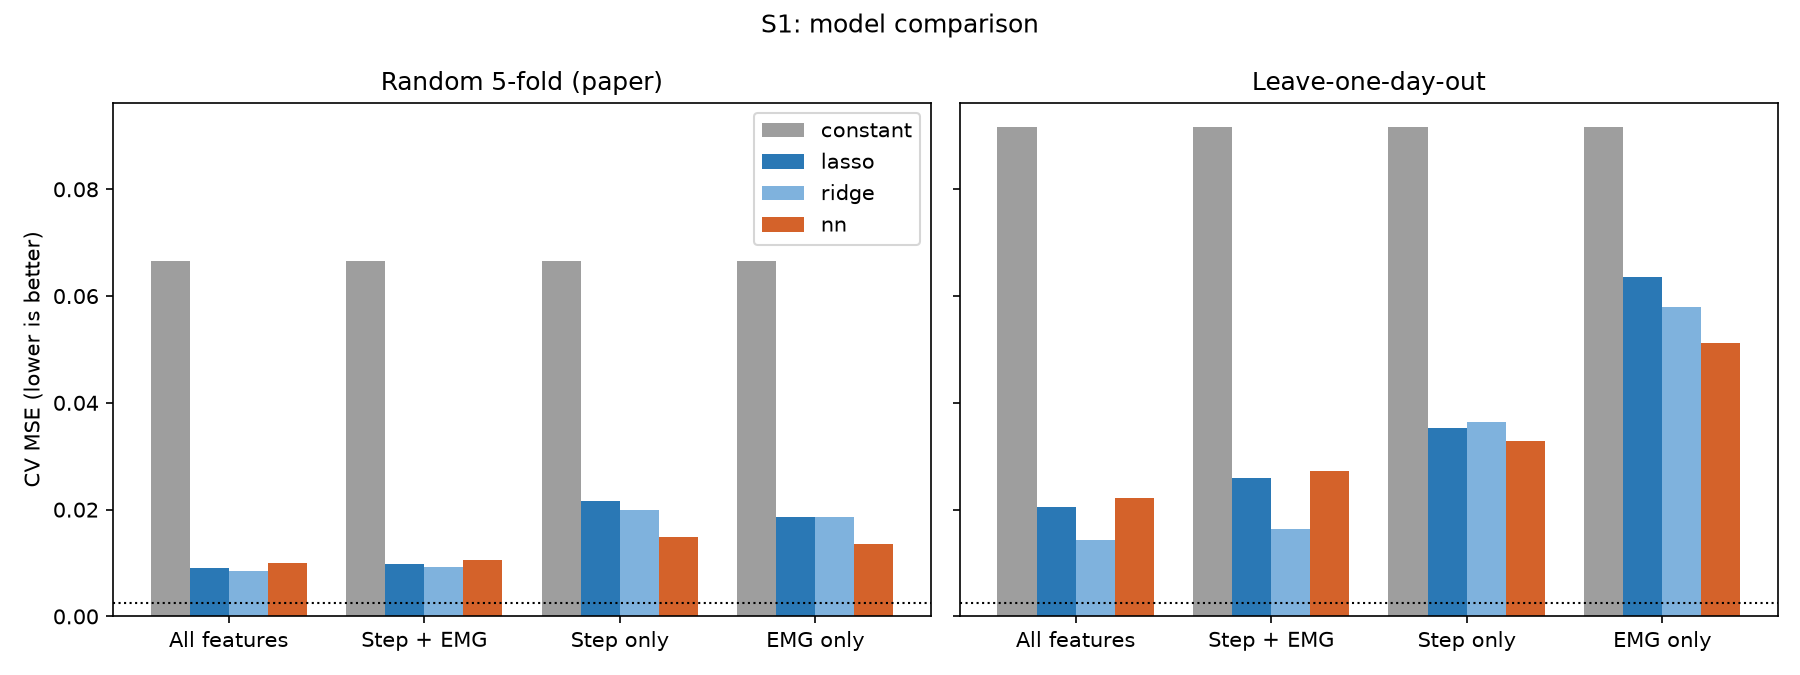
\includegraphics[width=\columnwidth]{figures/model_comparison_S1.png}
\vspace{-0.6cm}
\caption{S1: MSE per model and feature set under both protocols.}
\label{fig:cmp}
\end{figure}
\vspace{-0.3cm}

\textbf{Reproduction.} Under random k-fold our errors match the paper (S1 LASSO 0.0091 vs 0.0089,
an RMSE of about 10\% of normal-walking cost), and our nested-tuned NN improves on the paper's S2
network (0.0150 vs 0.0301).
\textbf{Unseen days.} LODO roughly doubles the error (S1 LASSO 0.0091$\to$0.0205; S2
0.0135$\to$0.0309); for S2 the best model explains only about 14\% of an unseen day's variance.
\textbf{Linear vs neural.} With all features, regularised linear models match the NN (best LODO:
Ridge 0.0143 for S1); the NN helps only on the small step-only and EMG-only sets, and larger
networks degrade under LODO.
\textbf{Features.} Step+EMG beats either group alone (Fig.~\ref{fig:cmp}). Control parameters help
markedly under LODO (S2 LASSO 0.0448$\to$0.0309), likely because the optimiser's settings drift
across days and encode adaptation. Nested forward selection (LODO MSE $\approx0.046$) and PCA did
not beat the full regularised models, and the selected features changed between held-out days.

\section{Conclusions}
We reproduced the reference accuracy in Python with a leak-free pipeline, and showed that the
headline numbers depend on the evaluation protocol: predicting a new walking day is roughly twice
as hard, because the subject's adaptation shifts metabolic cost from day to day. On 180 samples,
simple regularised linear models are as accurate as a shallow neural network. Future work: more
subjects, day-level normalisation or adaptation features, and evaluating on fully unseen subjects.
%% B-SECTIONS:END

\begin{thebibliography}{9}\small
\bibitem{krimsky} E. Krimsky and E. Ng, ``Predicting Metabolic Cost During Human-in-the-Loop
Optimization,'' CS229 Project Report, Stanford University, 2018.
\bibitem{zhang} J. Zhang \emph{et al.}, ``Human-in-the-loop optimization of exoskeleton
assistance during walking,'' \emph{Science}, 356(6344):1280--1284, 2017.
\end{thebibliography}

\noindent\small Code: private GitHub repository \texttt{hilo-metabolic-cost} (shared with faculty).
\end{document}
